\chapter{The evil in NAT}
\label{ch:nat}
\textbf{Network address translation}, or \textbf{NAT}, is a method of remapping an IP address space into another by modifying network address information in the IP header of packets while they are in transit across a traffic routing device. The technique was originally used as a means to mitigate the IPv4 address exhaustion, since one Internet-routable IP address of a NAT gateway can be used to identify an entire private network. For this characteristic NAT is also often used to hide the internal network structure, although this is not an advantage for security.

In practice, a NAT hides an entire IP address space, usually consisting of private IP addresses, behind a single IP address in a public address space (the NAT's). The hidden addresses are changed into a single public IP address as the source address of the outgoing IP packets so they appear as originating not from the hidden host but from the routing device itself.

In order to make NAT work, some IPv4 addresses have been declared \textit{private}\footnote{A private network is a computer network that uses private IP address space (RFC 1918). Being private by definition, these addresses cannot be used for routing in public networks, because they might be (actually, surely are) duplicate.} (see table \ref{tab:ipv4_private}; the most useful range is \textbf{class C}).

\begin{table}[h]
    \centering
    \begin{tabular}{|c|c|}
        \hline
        \textbf{Class} & \textbf{Address range} \\
        \hline
        A & \texttt{10.0.0.0} \\
        B & \texttt{172.16.0.0} \\
        C & \texttt{192.168.0.0} \\
        \hline
    \end{tabular}
        \caption{IPv4 private address space.}
        \label{tab:ipv4_private}
\end{table}

Note that although NAT exists for both IPv4 and IPv6, in IPv6 it is not commonly used, so from now on it shall be implied that we only refer to the IPv4 version.

Spoiler alert: this is where I'm packing these notes with \textit{more} memes. Because I can.

\begin{figure}[h]
    \centering
    
\includegraphics[scale=0.2]{img/unlimited_power_meme.jpg}
    \decoRule
    \caption{How I feel inserting memes in the notes.}
    \label{fig:meme_unlimited_power_nat}
\end{figure}

% TODO Find out if I can insert this masterpiece meme.
%\begin{figure}[h]
%    \centering
%    
\includegraphics[scale=0.5]{img/power_pec_meme.png}
%    \decoRule
%    \caption{How I feel inserting memes in the notes.\\
%    \footnotesize \textit{Credits for this masterpiece go to Abdullah Chaudhry. No offense intended (really).}}
%    \label{fig:power_pec_meme_nat}
%\end{figure}

%----------------------------------------------------------------------------------------

\section{NAT classification}
\label{sec:nat_class}
We can define three kinds of NATs:

\begin{itemize}
    \item \textbf{static NAT} (1:1 mapping): a single address in the private pool is directly translated to the public pool, using a stateless table; basically useless, because it does not save addresses: we need as many global addresses as the devices in the local network;
    \item \textbf{dynamic NAT}: dynamically maps an address in the private area network to another address of the outside area, meaning that only devices that are actually active need a binding (an active translation); for this reason, it needs a stateful table in order to track down which devices need to get outside of the network (and which not);
    \item \textbf{NAPT}, \textbf{Network Address and Port Translation}: the system does not only change the IP number, but also the layer 4 address (the TCP or UDP port), meaning that with a single global address we can actually host and keep up something like 64.000 connections (\textit{connections}, not hosts). In this case the system is a lot more complex, because it needs to track the single end-to-end connections (the \textbf{flow}) between devices in the private network and global network.
\end{itemize}

%----------------------------------------------------------------------------------------

\section{NAPT: Network Address and Port Translation}
\textbf{NAPT}, \textbf{Network Address and Port Translation}, represents the actual NAT that can be found in most private networks. As briefly explained in section \ref{sec:nat_class}, it is a variant of the dynamic NAT that tracks flows. A \textbf{flow} is identified in TCP/IP (in both TCP and UDP) by a five-tuple made of the \textit{protocol}, the destination and source \textit{IP addresses} and the destination and source \textit{ports}. We can differentiate between two flows by a change in any of these five elements. The protocol, destination IP and port cannot actually change, except for the source address and port which are modified by a NAT.

%-------------------------------------------

\subsection{NAT and cryptography}
\textit{Timete Danaos et dona ferentes}\footnote{\textit{Beware of Greeks bearing gifts.}}: NAT violates the non-modification principle of a package. Since it changes the IP addresses and ports, we will have to
re-compute the header and the TCP/UDP checksums, and previous data that could enable us to check if a packet has been tampered with will not be usable anymore. For this reason, the IPsec protocol does not work in NAT environments: all packets would be discarded due to a failure to the security check.

\begin{figure}[h]
    \centering
    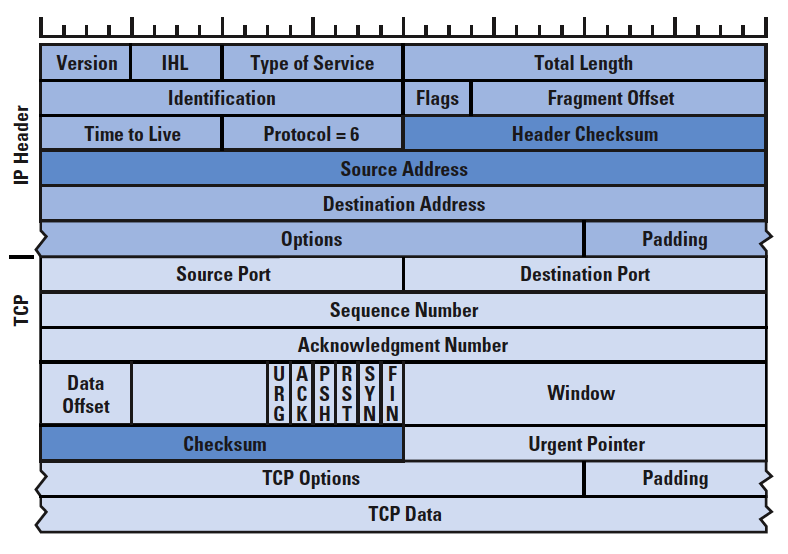
\includegraphics[scale=0.6]{img/ip_header.png}
    \decoRule
    \caption{A detailed diagram showing the IP and TCP header.}
    \label{fig:ip_header}
\end{figure}

\begin{figure}[H]
    \centering
    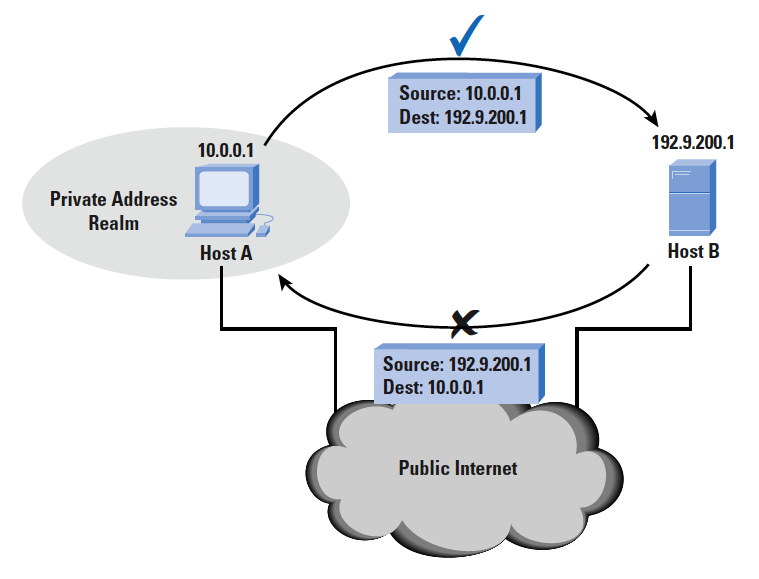
\includegraphics[scale=0.6]{img/nat_basic.png}
    \decoRule
    \caption{Using a private address to send something will get packets to their destination, but the receiver will not be able to respond to a private IP address.}
    \label{fig:nat_basic}
\end{figure}

The only way to do a checksum integrity check while using a NAT is to do it either after having passed the NAT, or inside the private network behind the NAT. An alternative, but extremely penalizing way (in terms of efficiency), is \textbf{IP-over-IP}, a technique which encapsulates an IP packet into another IP packet, so that it has two headers; we could also use \textbf{IP-over-TCP}, but all in all it kills the whole data transfer process.

%-------------------------------------------

\subsection{NAT basics}

As shown in figure \ref{fig:nat_basic}, it is also the NAT's job to change the IP header of incoming packets so as to deliver them to their intended receivers. The whole process is (usually) completely transparent to the user, and can be summarized as follows:

\begin{itemize}
    \item a packet arrives in the \textbf{internal interface} of the NAT:
        \begin{enumerate}
            \item search for a binding (a translation); does it exist?
                \begin{itemize}
                    \item \textbf{yes}: go to the next step;
                    \item \textbf{no}: create a binding;
                \end{itemize}
            \item translate the packet;
            \item forward the packet.
        \end{enumerate}
        
    \vspace{0.5em}
        
    \item a packet arrives in the \textbf{external interface} of the NAT:
        \begin{enumerate}
            \item search for a binding (a translation); does it exist?
                \begin{itemize}
                    \item \textbf{yes}: go to the next step;
                    \item \textbf{no}: \textit{drop} the packet;
                \end{itemize}
            \item translate the packet;
            \item forward the packet.
        \end{enumerate}
\end{itemize}

%----------------------

\begin{figure}[h]
    \centering
    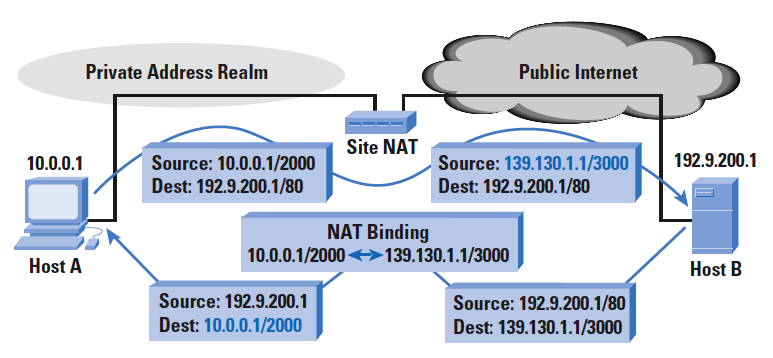
\includegraphics[scale=0.6]{img/nat_binding.png}
    \decoRule
    \caption{An example of NAT binding in a simple network.}
    \label{fig:nat_binding}
\end{figure}

\subsubsection{Bindings}
A \textbf{binding} is an entry in the NAT table that binds an internal protocol and IP to an external protocol and IP, basically specifying how to translate such a tuple:

\begin{center}
    \{IP, protocol, port\} \textit{(internal)} $\iff$ \{IP, protocol, port\} \textit{(external)}
\end{center}

It is not easy to determine if a binding is not needed anymore, so bindings have an expiration time; note that some of them can be deleted before their time expires: for example, since TCP flows can be closed gracefully, the NAT just waits for the final handshake and then removes the binding. NAT allows for 64.000 simultaneous bindings per protocol.

%----------------------

\subsubsection{Filters}
NAT \textbf{filters} decide if a packet should be translated, even if there is a binding for it. They make NAT \textbf{non-deterministic} (multiple behaviours, both good and bad), and they exist because of UDP:

\begin{itemize}
    \item \textbf{TCP} (one-on-one, two-way connection): sends and receives packets only to and from one endpoint, after a connection is established. Broadcast packets cannot be received, so every TCP packet will be translated by a NAT. TCP uses timeouts, making the connection expire after a certain time has passed since the last data has been received;
    \item \textbf{UDP} (data-based, connectionless): can receive from multiple senders without a previous connection, and broadcast meassages are allowed. It cannot be bound because there is no flow: it is not possible to decide when to delete a binding and a filter just by looking at the incoming/outgoing packets. It also introduces the demultiplexing problem: the NAT has to figure out which packet belongs to which flow, because there is only one socket (we need to ask the IP and UDP headers of the packet to check address and port).
\end{itemize}

%----------------------------------------------------------------------------------------

\section{NAT behaviours}
It is clear that the NAT must have different behaviours for TCP and UDP  - and what is worse, applications might not (properly) work if the "wrong" behaviour has been chosen. Here we describe the four types of NAT behaviour:

\begin{itemize}
    \item \textbf{symmetric NAT};
    \item \textbf{full cone NAT};
    \item \textbf{restricted cone NAT};
    \item \textbf{port restricted cone NAT}.
\end{itemize}

\begin{figure}[h]
    \centering
    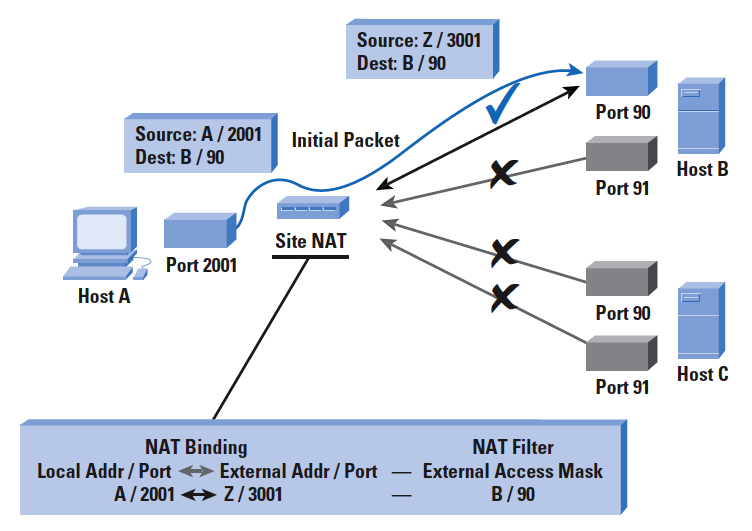
\includegraphics[scale=0.6]{img/symm_nat.png}
    \decoRule
    \caption{Symmetric NAT example.}
    \label{fig:symm_nat}
\end{figure}

%-------------------------------------------
\subsection{Symmetric NAT}
A \textbf{symmetric NAT} (fig. \ref{fig:symm_nat}) is one where all requests from the same internal IP address and port, to a specific destination IP address and port, are mapped to the same external IP address and port. If the same host sends a packet with the same source address and port, but to a different destination, a different mapping is used. Furthermore, only the external host that receives a packet can send a UDP packet back to the internal host. It works the same way for both TCP and UDP, and this is actually the only NAT behaviour used for TCP.

%-------------------------------------------
\subsection{Full cone NAT}
\begin{figure}[h]
    \centering
    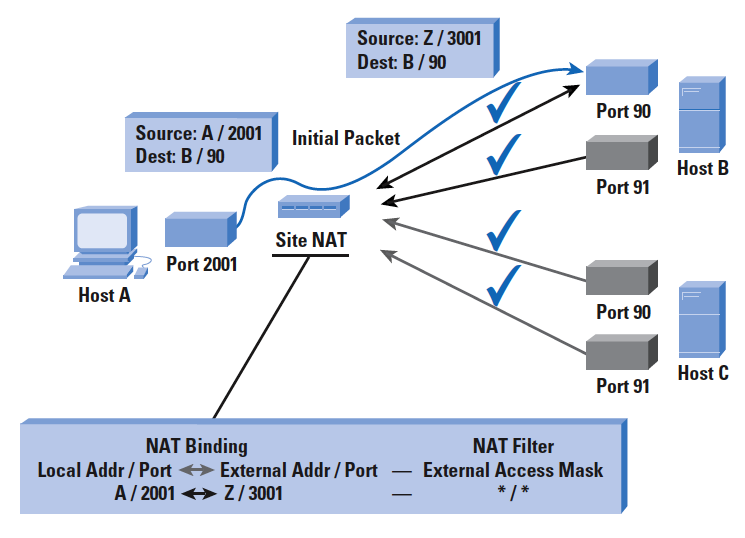
\includegraphics[scale=0.6]{img/full_cone_nat.png}
    \decoRule
    \caption{Full cone NAT example.}
    \label{fig:full_cone_nat}
\end{figure}

A \textbf{full cone NAT} (fig. \ref{fig:full_cone_nat}), the most common type of NAT, is one where all requests from the same internal IP address and port are mapped to the same external IP address and port. Furthermore, any external host can send a packet to the internal host, by sending a packet to the mapped external address. Depending on the filter, all other bindings can lead to a full cone NAT.

The security issue with this kind of NAT is that anybody can do a quick scan of the NAT server and will find which computers have something open: executing a network scan behind our network becomes a joke.

%-------------------------------------------
\subsection{Restricted cone NAT}
In a \textbf{restricted cone NAT} (fig. \ref{fig:restr_cone_nat}) all requests from the same internal IP address and port are mapped to the same external IP address and port. Unlike a full cone NAT, an external host (with IP address $X$) can send a packet to the internal host only if the internal host had previously sent a packet to IP address $X$. This kind of NAT is slightly better than a symmetric NAT, but for practical purposes is kinda useless because referral and handover\footnote{\textbf{Handover} or \textbf{handoff} is the process of transferring an ongoing data session from one channel connected to another (e.g. when a phone moves away from an area covered by one cell and enters an area covered by another cell, the call is transferred to the second cell in order to avoid call termination).} do not work.

\begin{figure}[h]
    \centering
    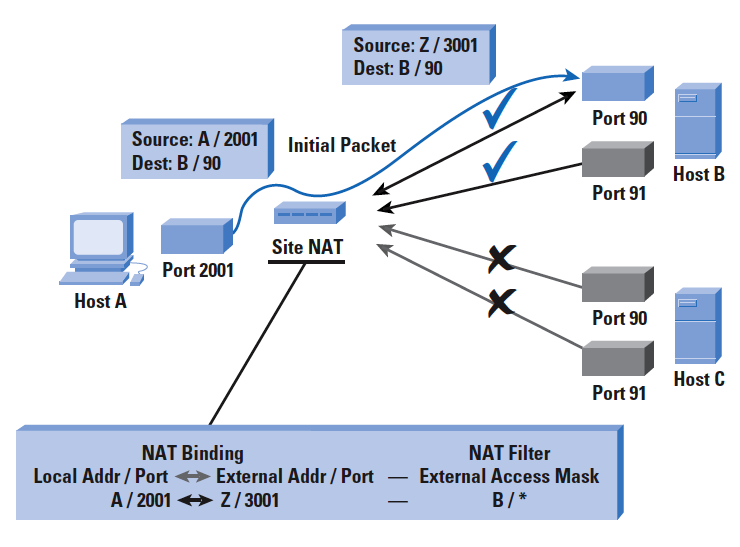
\includegraphics[scale=0.6]{img/restr_cone_nat.png}
    \decoRule
    \caption{Restricted cone NAT example.}
    \label{fig:restr_cone_nat}
\end{figure}

\begin{figure}[H]
    \centering
    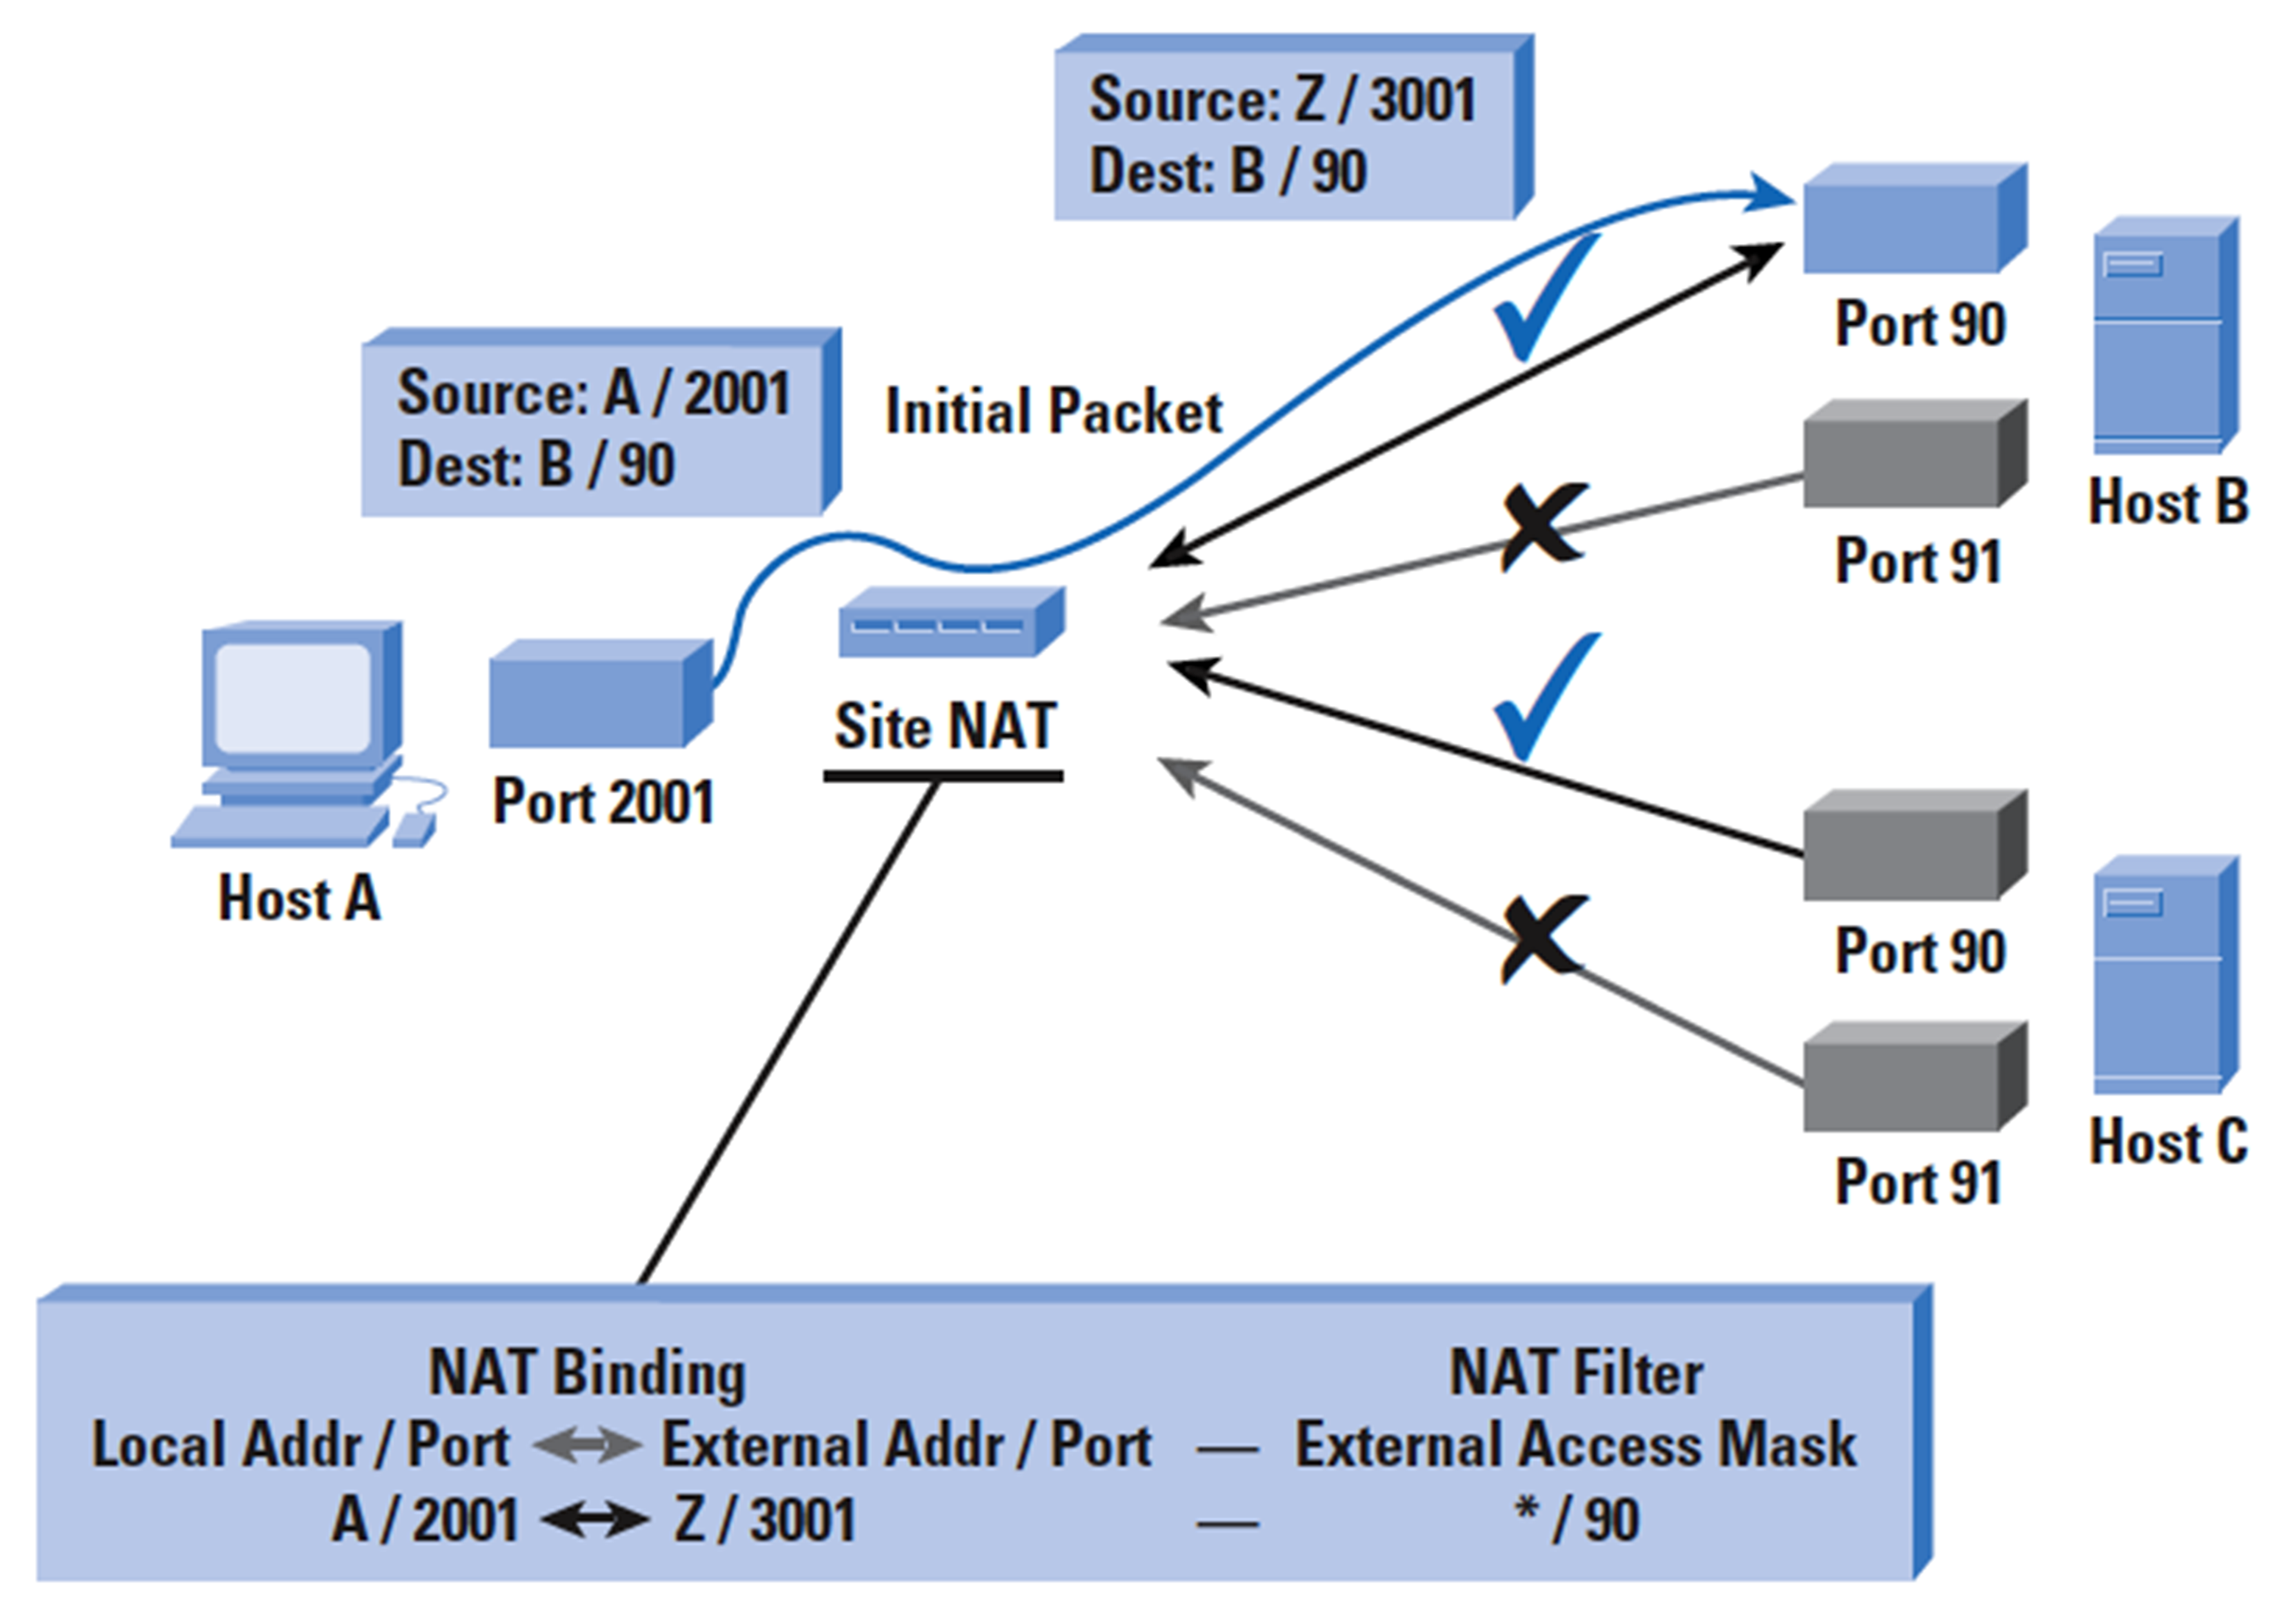
\includegraphics[scale=0.13]{img/port_restr_cone_nat.png}
    \decoRule
    \caption{Port restricted cone NAT example.}
    \label{fig:port_restr_cone_nat}
\end{figure}

%-------------------------------------------
\subsection{Port restricted cone NAT}
A \textbf{port restricted cone NAT} (fig. \ref{fig:port_restr_cone_nat}) is like a restricted cone NAT, but the restriction includes port numbers. Specifically, an external host can send a packet, with source IP address $X$ and source port $P$, to the internal host only if the internal host had previously sent a packet to IP address $X$ and port $P$.

In this kind of NAT we can still do a network scan if we know the port that must be used as source port, in order to send packets to the NAT and then have them translated towards the internal computer. However, there are more chances that the NAT or the firewall will spot suspicious activity. For this reason, UDP should be used only with this NAT behaviour.

%-------------------------------------------
\subsection{Hairpinning}
\textbf{Hairpinning} (or NAT loopback, see figure \ref{fig:hairpin}) describes a communication between two hosts behind the same NAT device using their NAT-mapped endpoint. Because not all NAT devices support this communication configuration, applications must be aware of it.

In other words, hairpinning is where a machine on the LAN is able to access another machine on the LAN via the external IP address of the LAN/router (with port forwarding set up on the router to direct requests to the appropriate machine on the LAN). 

This ability of the NAT is relevant in cases where there is a host that wants to reach another host behind the same NAT, but it only knows its (the destination's) public address.

\begin{figure}[h]
    \centering
    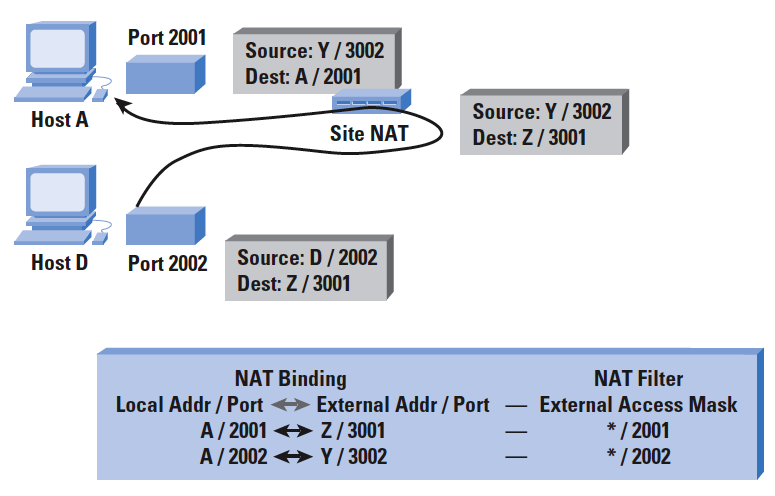
\includegraphics[scale=0.6]{img/hairpin.png}
    \decoRule
    \caption{NAT loopback (hairpinning) example.}
    \label{fig:hairpin}
\end{figure}

%-------------------------------------------
\subsection{STUN}
Sometimes we need to find out what kind of NAT we have, so that we can know if we can use certain applications. \textbf{STUN}\footnote{Rosenberg, J., Weinberger, J., Huitema, C., and R. Mahy, \textit{STUN - Simple Traversal of
User Datagram Protocol (UDP) Through Network Address Translators (NATs)}, RFC 3489, March 2003.} is just the tool for that.

STUN is a \textbf{request-reply protocol}: \textit{server, where did this packet come from?} The server replies, and STUN infers the NAT type from the answer, as shown in figure \ref{fig:stun}.

\begin{figure}[h]
    \centering
    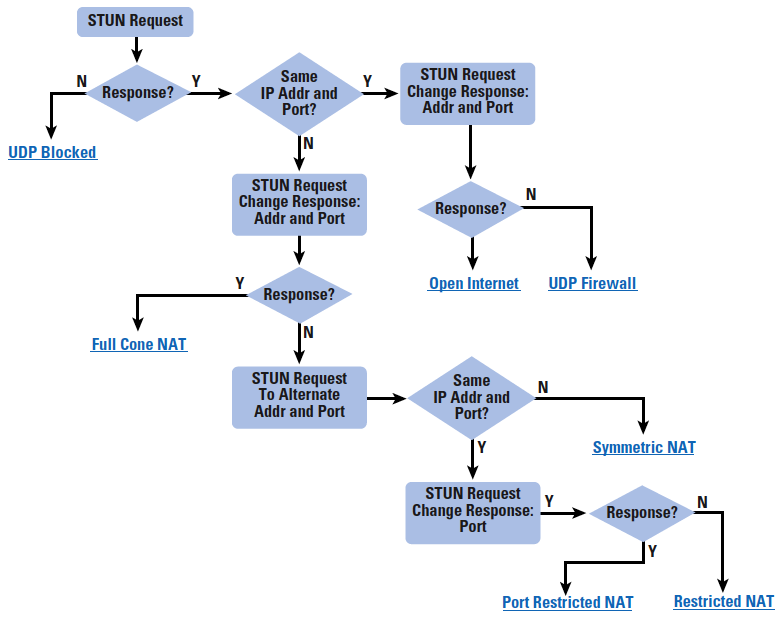
\includegraphics[scale=0.7]{img/stun.png}
    \decoRule
    \caption{STUN NAT characterization algorithm.}
    \label{fig:stun}
\end{figure}

In order to make a STUN request we need a STUN server hosted on a computer which has two global IP addresses with two open ports for each address (a capability of four total connections). The client, typically operating inside a private network, sends a binding request (through a UDP packet) to a STUN server on the public Internet. The STUN server responds with a success response that contains the IP address and port number of the client, as observed from the server's perspective.

\vspace{0.5em}

\emph{Example} Let us consider the full cone NAT shown in figure \ref{fig:full_cone_nat}. If host C can reach us from port 90, then the only possibility is that we have a full cone NAT, because that connection is only allowed in full cone; if we do not receive an answer, then we ask to use what remains (a restricted cone or port NAT). At the end of the day we can discriminate between all types of NATs.

\vspace{0.5em}

STUN is not reliable. First of all, since UDP does not provide reliable transport guarantees, a certain level of reliability is achieved by application-controlled retransmissions of the STUN requests. However, NATs are non-deterministic, meaning that their behavior can change over time; also a client might have multiple NATs one behind the other (this actually happens a lot more than one might think): in this cases, STUN might just outright fail.

%----------------------------------------------------------------------------------------

\section{More NAT classification}
\begin{figure}[h]
    \centering
    
\includegraphics[scale=0.5]{img/more_meme.png}
    \decoRule
    \caption{Did you really think we were done with NAT classification? Wrong! MORE!}
    \label{fig:more_nat_meme}
\end{figure}

Now, let us clear the fact that in order to \textit{really} classify a NAT we have to check its bindings and filters. Take for example the system shown in figure \ref{fig:wut_nat}, where the NAT maps the host into two completely different things: what kind of NAT is this?\footnote{Spoiler: a shitty one.}

\begin{figure}[h]
    \centering
    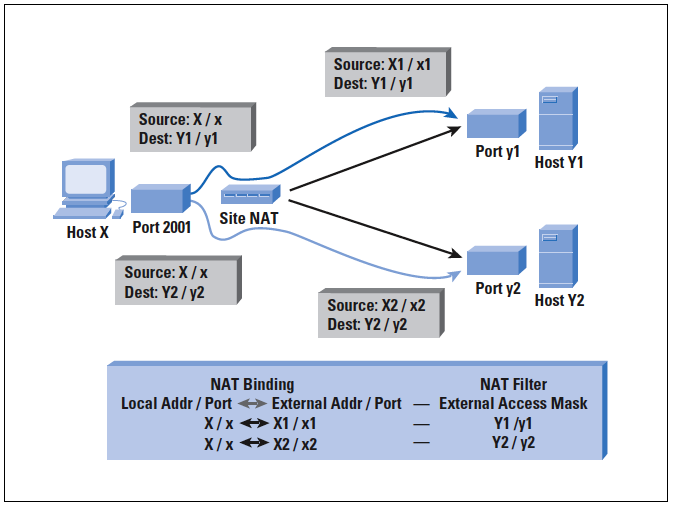
\includegraphics[scale=0.6]{img/wut_nat.png}
    \decoRule
    \caption{How the f- do we classify \textit{this}?}
    \label{fig:wut_nat}
\end{figure}

%-------------------------------------------

\subsection{Binding}
\label{nat:binding_2}
NAT bindings can belong to one of these four types:

\begin{itemize}
    \item \textbf{endpoint independent}: the NAT re-uses the binding for all packets with the same source IP/port. The
destination IP/port is not considered (full cone NAT);
    \item \textbf{endpoint address dependent}: the NAT re-uses the binding for all packets with the same source IP/port and destination IP. The destination port is not considered (restricted cone NAT);
    \item \textbf{endpoint port dependent}: the NAT re-uses the binding for all packets with the same source IP/port, and destination port. The destination IP is not considered (port restricted cone NAT);
    \item \textbf{endpoint address and port dependent}: the NAT re-uses the binding for all packets with the same 5-tuple (symmetric NAT).
\end{itemize}

%-------------------------------------------

\subsection{Port binding}
NAT port bindings can belong to one of these three types:

\begin{itemize}
    \item \textbf{port preservation}: the NAT tries to not change the port number. If two (or more) hosts use the same source port, all but the first one will have their port changed;
    \item \textbf{port overloading}: same as port preservation, the second host will win, and the binding of the first one will be discarded (ouch);
    \item \textbf{port multiplexing}: the NAT does aggressive multiplexing, trying to multiplex flows over the same port
according to the destination address/port. It can cause a lot of issues if some hosts try to connect with the same destination host. The NAT must figure out when to do multiplexing and when not to do it.
\end{itemize}

In conclusion, it is (almost) impossible to predict what the NAT will do. This is why programs usually reserve several ports (about 10-15), but it is neither logical, nor efficient or secure because every open binding allows data to go back to the sender.

%-------------------------------------------

\subsection{Timer refresh}
A NAT timer can be refreshed in the following ways:

\begin{itemize}
    \item \textbf{bidirectional}: the timer is refreshed by incoming \textit{and} outgoing packets;
    \item \textbf{outbound}: only outgoing packets will refresh the timer; depending on the application, a
keep-alive might be needed;
    \item \textbf{inbound}: only incoming packets will refresh the timer; depending on the application, a
keep-alive might be needed;
    \item \textbf{Transport Protocol state}: this one tries to decode the application-level protocol and "do the right thing" – which it often does not.
\end{itemize}

Note that all but outbound timer refreshes lead to DoS attacks. Bidirectional or inbound refreshes are not recommended because an attacker could snoop which flows are active, then keep sending packets to their bindings: perhaps those dataframes will be discarded, but in the meantime the bindings will be kept alive. This is a great way to starve the NAT to death (panic attacks).

Outbound refresh is good until we use it for streaming stuff, because we will have to send keep alive packets from the side that is not the main sender (for example the host will have to say to Netflix that is still alive, otherwise the binding will timeout - even though it is Netflix the one sending shitloads of data packets). UDP is unidirectional, so this method will not work. As for the Transport Protocol state, it has to know what is the state of a layer 7 application: the NAT can do that, and it will,  but it needs to know the protocol of the application, and layer 7 protocols are not always open source (some of them are standard and public, but many others, like Skype or Webex, are private and copyrighted, and cannot be simply reverse-engineered).

%-------------------------------------------

\subsection{External filtering}
NAT filtering includes the following modes (the same as the bindings in section \ref{nat:binding_2}):

\begin{itemize}
    \item \textbf{endpoint independent}: does not do anything (full cone NAT);
    \item \textbf{endpoint address dependent}: filter based on destination IP (restricted cone NAT);
    \item \textbf{endpoint address and port dependent}: filter based on destination IP \textit{and} port (symmetric NAT).
\end{itemize}

Remember that filters and bindings must be paired, but can behave in completely different ways. We cannot check to which category belongs the binding or port that we are using; everything depends on the amount of resources (CPU/memory) of the NAT, which will change during the day.

\begin{figure}[h]
    \centering
    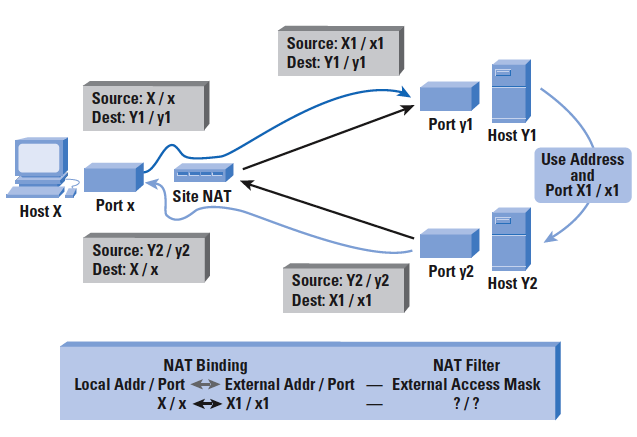
\includegraphics[scale=0.7]{img/nat_ext_filtering.png}
    \decoRule
    \caption{NAT external filtering.}
    \label{fig:nat_ext_filtering}
\end{figure}

%----------------------------------------------------------------------------------------

\section{NAT: conclusions}

%-------------------------------------------

\subsection*{P2P applications}
\textbf{Peer-to-peer}  (\textbf{P2P}) computing or networking is a distributed application architecture that partitions tasks or workloads between peers which are equally privileged, equipotent participants in the application. Nowadays every damn thing in a house that tries to be "smart" uses this technology (NAS (Network Attached Storage), smart TV and similar),  because it opens ports on the NAT, using NAT traversal techniques, since they make it easier for the user to check these devices quickly. This also means, however, that an attacker can do the same.

Basically, every binding that is open allows packets to flow back to the host; the most extreme cases happen when we have started a communication days ago and still have a binding active because of this behaviour, which makes it very dangerous.

%-------------------------------------------

\subsection*{ICMP, layer 3 encryption \& co.}
All packets that do not have specific ports, like in \textbf{Internet Control Message Protocol} (\textbf{ICMP}) messages, work by magic: instead of opening a port, they use a specific binding for that computer. If we are behind a NAT and try to send a ping to another host behind another NAT, we can do it (one device at a time).

%-------------------------------------------

\subsection*{IP fragmentation}
In order to translate packets we have to check the layer 4 header, but fragments do not contain this layer (because it only appears in the first packet). For this reason, NATs have to check the fragment ID or reconstruct the fragment. Either cases are not very nice: fragment ID needs an even more complex machine, and rejoining the packet inside the NAT introduces latency, more memory requirements, and in the end the risk of resource starvation.

%-------------------------------------------

\subsection*{UPnP and IGD}
An \textbf{Universal Plug and Play} (\textbf{UPnP}) compatible device from any vendor can dynamically join a network, obtain an IP address, announce its name, convey its capabilities upon request, and learn about the presence and capabilities of other devices.

The problem with this one is self-explaining: UPnP allows a program/host/application to forcefully open a binding, meaning that the application can ask the NAT to assign them a specific port - which in turn leads to having specific and very well known ports (not only by us, but also by attackers) permanently open on the NAT.

The \textbf{Internet Gateway Device Standardized Device Control Protocol} (\textbf{IGD}) worsens the situation as it allows an UPnP device to discover the external IP address used by the NAT and to automatically create bindings and filters.